\section{Module Implementation}\label{ModuleImp}
This section implements the modules that are specified in section \ref{ModuleDes}. In subsection \ref{VirtEnvStat} the scene in the Unity3d game engine is modelled with static elements such as the terrain and objects. This is followed by the design of the dynamic elements that are navigated through the scene e.g. a vessel and different sensors (\ref{VirtEnvDyn}). A third subsection \ref{DataProcessing} details the \ac{ROS} network that is programmed to process the data of the sensors in the Unity3d scene.

\subsection{Static environment} \label{VirtEnvStat}
% The code level, pseudo code in the modules, most detailed description.
In a first step, the virtual scene is modelled in Unity3d running on Linux 20.04 LTS. As a geographic reference for the terrain, the location proposed for the physical implementation of the project \ac{ELLA} is used. Elevation data for this location in the reference coordinate system EPSG 25832 for the position and EPSG 7837 for the height from east 384999 to west 383000 and from north 5720999 to south 5719000 is provided in .xyz data by OpenDataNRW with a resolution of one meter \cite{Xyzdata}.\\

The data is loaded into to the software QGIS Version 3.16.6 LTR. QGIS is an open source geographic information system and provides various functionalities in this domain. One of them is the creation of a \ac{TIN} which can represent a \ac{DEM}. Given a function $z = f(x,y)$ in which $x$ and $y$ represent the position data and z the according height, the function can be computed only for discrete points as $x$ and $y$ are finite in $S$ and depend on the resolution of the source. Therefore, in order to map the \ac{DEM} continuously, a \ac{TIN} has to be created that connects the discrete points so that they suffice three conditions. First the number of vertices $T$ of the resulting triangles have to be equal to the number of points $S$. As a second condition the interiors of the triangles out of $T$ are not allowed to intersect each other and if the boundaries of two triangles intersect each other, the intersection has to be either a common edge or a common vertices. On the resulting triangles, a linear interpolation function can be applied and thus a continuous \ac{DEM} approximation is achieved \cite{TIN}.\\

To convert the \ac{DEM} to a .raw heightmap that is used by Unity3d to create a terrain, the \ac{DEM} is converted to a .TIFF and exported to Gimp. Gimp is an open source image manipulation program and supports various file formats of which the .raw format is one. The resulting image is shown in figure \ref{fig_HenrichHeight}. On a 256-bit greyscale resolution the darker regions of the image represent low terrain with increasing height for every step towards white. With the import function of Unity3d the terrain is then shaped according to the heightmap. The resulting terrain data is visualized in figure \ref{fig_terrainRaw}. The sink in the bottom-left of the image matches the second dark shape along the top of figure \ref{fig_HenrichHeight}.\\ 
\begin{figure}[!htb]
	\begin{minipage}[t]{0.48\textwidth}
		\centering
		\includegraphics[width=.99\linewidth]{Bilder/Henrich_SE.jpeg}
		\caption{Height map of the scene that is to be modelled}\label{fig_HenrichHeight}
	\end{minipage}\hfill
	\begin{minipage}[t]{0.48\textwidth}
		\centering
		\includegraphics[width=.99\linewidth]{Bilder/terrainRaw.png}
		\caption{Terrain data in Unity3d derived from a height map}\label{fig_terrainRaw}
	\end{minipage}
\end{figure}

Another option to create a terrain out of the \ac{DEM} is represented by importing the data into blender and create a mesh that is then exported to Unity3d as an object. However it turned out that the advantage that comes with the possibility of granular mesh manipulation is at the same time a disadvantage. A highly intersected mesh with a very large amount of vertices can not be easily joined without destroying the integrity of the mesh, that is the consistency of vertices connections. Thus the larger the area that is modelled and the more details in terms of position resolution is required, the less manageable the mesh becomes in terms of processing time required for visualization.\\

The terrain as shown in figure \ref{fig_terrainRaw} is smoothed which is necessary because of the limited resolution of the height map that is restricted to 256-bit on the greyscale that represents the height. On the resulting terrain, a satellite image of the scene serves as a background texture. Various other textures are then applied to the scene to resemble the real environment. In the software Blender 2.92.0, 3D objects are created and imported into the virtual environment. As the process of creating the objects and applying textures and shader as well as collision meshes to the objects is rather tedious, only objects that are vital to the scene are modelled. For reasons of simplicity only rigid bodies are used in the scene. Rigid bodies are volume bodies in which every set of two different arbitrary points contained in the body have the same distance to each other at any time. Figure \ref{fig_smallvessel} shows the Blender model of the small vessel that is used in the Unity3d scene. It is composed of multiple connected objects that can be used to derive a collision mesh from. The collision mesh surrounding the vessel inside the modelled scene is depicted in figure \ref{fig_collisionmesh} with the mesh coloured in green. There are two option for the generation of the mesh in Unity3d. A concave mesh takes the vertices inside the object and a convex mesh is laid over the vertices outside. The collision mesh as depicted is a convex shape. It can be noted that there are differences of the mesh to the shape of the visible object that results of the inability of the mesh to project on concave and convex parts in the same object.\\

 	\begin{figure}[!htb]
 	\begin{minipage}[t]{0.48\textwidth}
 		\centering
 		\includegraphics[width=.99\linewidth]{Bilder/BlenderVessel.png}
 		\caption{Blender vector model of a small vessel used in the modelled scene}\label{fig_smallvessel}
 	\end{minipage}\hfill
 	\begin{minipage}[t]{0.48\textwidth}
 		\centering
 		\includegraphics[width=.99\linewidth]{Bilder/CollisionmeshVessel.png}
 		\caption{Small vessel with collision mesh generated from the blender model}\label{fig_collisionmesh}
 	\end{minipage}
 \end{figure}

The scene as seen from above is shown in figure \ref{fig_UnityBird}. The V-shaped river is in the center of the image with a total of five landing stages and two small vessel located on it. With a satellite image as a background, texures for paths, meadows and the rivers shore are applied on the terrain. Trees and houses further detail the scene. The water is represented by a mesh of Unity3d's standard assets. The standalone application that can be run without a Unity3d IDE can be seen in figure \ref{fig_UnityPerson}. Settings in the top left of the application allows for the change of perspective out of which the scene is rendered, the change of resolution and for reloading or closing the scene. In the foreground the small vessel on which the sensors are mounted can be seen. In the background, the aforementioned textures and objects are visible.
 \begin{figure}[!htb]
 	\begin{minipage}[t]{0.48\textwidth}
 		\centering
 		\includegraphics[width=.99\linewidth]{Bilder/UnitySceneBird.png}
 		\caption{Unity3d scene from above}\label{fig_UnityBird}
 	\end{minipage}\hfill
 	\begin{minipage}[t]{0.48\textwidth}
 		\centering
 		\includegraphics[width=.99\linewidth]{Bilder/UnitySceneFirstPerson.png}
 		\caption{Unity3d with menu from sensor perspective}\label{fig_UnityPerson}
 	\end{minipage}
 \end{figure}



\subsection{Dynamic Environment} \label{VirtEnvDyn}

With the scene modelled, defining its behaviour during runtime is the next step. To obtain a realistic physics simulation, Unity3d makes use of a physics engine. The main task of a physics engine is to solve forward dynamics, however there are many factors that determine the performance of a physics engine and thus there are many different implementations available. Collision and energy restitution, the modelling of constraints and the integrator performance are among the factors that can be evaluated in order to determine a suitable implementation. Unity3d default physics engines are PhysX supplied by Nvidia and Havok Physics supplied by Havok. It has to be noted, that both engines are optimized towards the appliance in games and therefore a strong focus is on the engines stability rather then the accuracy \cite{PhysXComp}. In Unity3d, the physics module provides an abstraction level to access functions related to 3D physics. These functions are used among others to steer a small vessel with a keyboard input through the scene. The forward movement and the rotation of the vessel are taken as an input and serve the purpose of altering the position of the virtual sensors that are mounted on the vessel.\\

All data types of the sensors are saved in a central script called Sensor Manager. For every sensor instance, a public data storage class is instantiated that can be accessed by the sensor class as well as by the class that sends the data to the \ac{ROS} network. The foundation of what is used as a \ac{LIDAR} sensor and \ac{IMU} sensor in Unity3d is already defined. Only the saving process is changed to allow an adaptation to the outlined data exchange method. The \ac{LIDAR} sensor class makes use of the so called raycast, which is one method provided by the physics engine to provide scene queries. A point cloud in the scenes global coordinate system results of the colliders that are hit by the emitted rays. Various variables such as the field of view and the sweep frequency allow for the simulation of physical implemented sensors. To transmit the pointcloud, its three-dimensional cartesian positional data is saved with one list for each dimension. A list with an altering size for each cycle comes with the disadvantage of a required memory allocation for every measurement cycle. However, as the data size of the pointcloud is changing depending on the objects that are hit by the raycast, a list allows for having the lowest data size possible.\\

Based on the physical operating principle of a real \ac{RADAR}, a virtual \ac{RADAR} is implemented in Unity3d as depicted in figure \ref{fig_radarrays}. The emittance of an electromagnetic wave of a real \ac{RADAR} is simulated by a discrete beam that consists of raycasts. As a sequential calculation of the collisions of objects with the emitted rays increases the process time and decreases the simulation performance, a job handle is used that is implemented in the \ac{LIDAR} sensor as well. A job handle allows for parallel execution of tasks and thus can increase the process time. The resolution of the discrete beams is adaptable with a variable in the script of the sensor. Each time an object is hit by the raycast, the positional data is saved together with a reflectance value of the object. The reflectance value is provided by a script that can be attached to objects to further detail its  material properties. That is useful especially for a \ac{RADAR} as the reflected energy not only results of the object size but of the objects material, too. After one turn that consists of a predetermined number of beams, the cartesian three-dimensional positional data of all detected objects is mapped to a two-dimensional space by omitting the height data.\\
\begin{figure}
	\begin{centering}
		\centering
		\includegraphics[width=0.6\linewidth]{Bilder/radarrays.png}
		\caption{Raycast of the radar with active rays visualized  in red}
		\label{fig_radarrays}
	\end{centering}
\end{figure}

To resemble the image of a radar, an array  is set up with the length resulting of the predetermined number of beams multiplied by the set cell extension in every beam. Starting at the center $M$ that is the sensor center, the array consists of the subsequent beams cell values. Each cell can be accessed with an index as shown in figure \ref{fig_radarPol} and is defined by its radius $r_{min}$ and $r_{max}$ and angle theta $t_{min}$ and $t_{max}$. The quantity $C$ of points inside the cell now follow equation \ref{eq_insideCell}. 
\begin{equation}
C = {r,t| r_{min}<r>r_{max} \wedge t_{min}<t>t_{max}}
\label{eq_insideCell}
\end{equation}
 The two-dimensional cartesian positional data is transformed to a quantity of polar coordinate representations called $P$. The points $I$ inside the cell now follow equation \ref{eq_PinsideCell}. 
\begin{equation}
	I = P \cap C
\label{eq_PinsideCell}
\end{equation}
The reflectance value $r$ of the each cell can be calculated with equation \ref{eq_RefinsideCell} with $ref_i$ being the aforementioned individual reflectance for each object. Each value can be saved to the array that can then be transmitted to the Sensor Manager.\\
\begin{equation}
% || = how many elements inside the quantity
r = \sum_{i=0}^{i=|I|} I_i * ref_i
\label{eq_RefinsideCell}
\end{equation}


 \begin{figure}
	\begin{centering}
		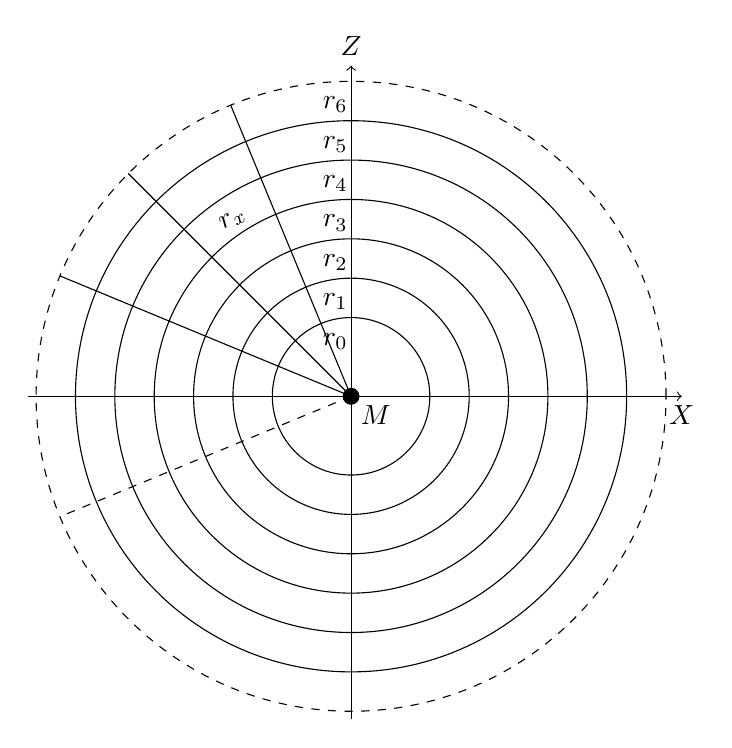
\begin{tikzpicture}      
		%\draw[help lines,xstep=.5,ystep=.5,dashed] (0,0) grid (10,10); %Hilfsdiagramm für Koordinaten
		%\foreach \x in {0,1 ,...,10} { \node [anchor=north] at (\x,0) {\x}; }
		%\foreach \y in {0,1,...,10} { \node [anchor=east] at (0,\y) {\y}; }
		
		\draw[->,] (0.9,5) -- 	(9.2,5) node  [at end,anchor= north]{$X$}; %x axis
		\draw[->,] (5,0.9) -- 	(5,9.2) node  [at end,anchor= south]{$Z$}; %z axis
		
		\draw[fill=black]       (5,5) circle (0.1) node (M)[below right]{$M$}; % point M
		
		\draw      (5,5) circle (1) node (M1){}; % first circle around center
		\draw      (5,5) circle (1.5) node (M2){}; % circle around center
		\draw      (5,5) circle (2) node (M3){}; % circle around center
		\draw      (5,5) circle (2.5) node (M4){}; % circle around center
		\draw      (5,5) circle (3) node (M5){}; % circle around center
		\draw      (5,5) circle (3.5) node (M6){}; % circle around center
		\draw [dashed]     (5,5) circle (4) node (M7){}; % last circle around center
		
		\draw[-,] (5,5) -- 	(3.47,8.7) node  [at end,anchor= north]{}; % 22.5 degree 
		\draw[-,] (5,5) -- 	(2.17,7.83) node  [at end,anchor= north]{}; % 45 degree 
		\draw[-,] (5,5) -- 	(1.3,6.53) node  [at end,anchor= north]{};% 67.5 degree
		\draw[dashed] (5,5) -- 	(1.3,3.47) node  [at end,anchor= north]{};% 115.5 degree
		
		
		\draw[fill=black]       (4.8,5.7) circle (0) node (C)[]{$r_0$}; % point 1
		\draw[fill=black]       (4.8,6.2) circle (0) node (C)[]{$r_1$}; % point 2
		\draw[fill=black]       (4.8,6.7) circle (0) node (C)[]{$r_2$}; % point 3
		\draw[fill=black]       (4.8,7.2) circle (0) node (C)[]{$r_3$}; % point 4
		\draw[fill=black]       (4.8,7.7) circle (0) node (C)[]{$r_4$}; % point 5
		\draw[fill=black]       (4.8,8.2) circle (0) node (C)[]{$r_5$}; % point 6
		\draw[fill=black]       (4.8,8.7) circle (0) node (C)[]{$r_6$}; % point 7
		\draw[fill=black]       (3.5,7.25) circle (0) node (C)[rotate=30]{$r_{x}$}; % point 1
		
		\end{tikzpicture}
		\caption{2D Cartesian and polar coordinates with index and reflectance value of \ac{RADAR} cells.}
		\label{fig_radarPol}
	\end{centering}
\end{figure}

To send sensor data to \ac{ROS}, a library for Unity3d called ROS\# is used. ROS\# can be integrated into Unity3d and makes use of the messages that are defined in \ac{ROS}1. As there are only few differences in the default messages provided by \ac{ROS}1 to the subsequent implementation \ac{ROS}2, the library can be used for both frameworks. However, it is noted that the message of type header makes use of a different notation for time units and thus has to be adjusted. In addition to default messages, \ac{ROS} provides the possibility to define custom messages that can then be exported to ROS\#. Custom messages in the context of the particular use case are derived from the sensor data classes. As a webbridge run by Node.js serves as an intermediary framework for data transmission, new messages types have to be introduced to it as well.\\

\subsection{Data processing} \label{DataProcessing}

New message transmitted to the \ac{ROS} network are first received by the nodes that process the message data. In \ac{ROS} nodes are executables that can communicate to other nodes with an interface such as datatypes defines in messages. To avoid stressing the network with high data rates, for large messages a design maxim in this project is the reduction of data size in the first node that receives the data. That can be done by algorithms that for example filter, cluster and segment data. \\

Figure \ref{fig_rqt} displays the structure of the data processing in \ac{ROS}. The node transform\_listener is not used as it is only relevant for coordinate system transformations that are not taking place in the scope of this work. The ros2\_web\_bridge-node connects to the programmed Unity3d scene and receives its messages. A total of four \ac{ROS} nodes that are named image\_subscriber, lidar1\_xyz, radar1\_img and get\_imu process the incoming data. After being processed, the lidar and radar data are published again and are received by the n\_rviz node that is a predefined \ac{ROS} visualization tool.  \\
\begin{figure}
	\centering
	\includegraphics[width=.99\linewidth]{Bilder/rviz2.png}
	\caption{Node and interface structure of ROS2 navigation package}
	\label{fig_rqt}
\end{figure}

The incoming \ac{IMU} data is not further processed but solely displayed as shown in figure \ref{fig_IMU}. The angular velocity in $x$,$y$ and $z$ as well as the acceleration information of the sensor is plotted in a time frame of five seconds. As in Unity3d the sensor is mounted on a object without further specified physical characteristics, the object acceleration in positive as well as negative direction is not further specified by properties such as weight. Presumably this accounts for the rapid changes in for example the acceleration in $x$ direction. The visualization makes use of the \textit{matplotlib} library for python with the plot style set to continuous plotting. It has to be kept in mind that the library as well as \ac{ROS} has its own event handling and resulting loop. Therefore, not every setting of \textit{matplotlib} can be used for plotting data together with \ac{ROS}. \\

The \ac{LIDAR} data that is received from the Unity3d scene has to be processed in order to extract obstacles that are used to map the environment. As there are many algorithms that operate on large datasets of three dimensional data, the approach that is best suited for the application has to be found. The Hough Transform Algorithm directly extract contours in the data it is applied on. That comes in handy as it requires no other processing. However as on every point of the data iterations are conducted, it can be expected that the method does not provide the performance used for realtime applications in which new data comes in at high intervals. The same drawback counts for the disqualification of the partition based K-Means clustering algorithm. Additionally, this algorithm only gets to local optimal solutions in a limited processing time. The hierarchic \ac{BIRCH} clustering algorithm tends to subdivide large cluster that in fact are intended to be viewed as one cluster. The last discussed algorithm is the density based \ac{DBSCAN} clustering algorithm. An advantage of this method is the detection of noise that can then be neglected for mapping the environment. This algorithms promises the best results as no disadvantages can be noticed. Thus it is applied in the node that clusters the \ac{LIDAR} data in an implementation that makes use of parallel procession of points \cite{ParaDBSCAN}. Figure \ref{fig_lidarMat} displays the segmented data. For example the coloured vertical lines can be classified as colliders of trees. Again, \textit{matplotlib} is used for the data visualization.\\
 \begin{figure}[!htb]
 	\begin{minipage}[t]{0.48\textwidth}
 		\centering
 		\includegraphics[width=.99\linewidth]{Bilder/IMU.png}
 		\caption{IMU data with acceleration and angular velocity}\label{fig_IMU}
 	\end{minipage}\hfill
 		\begin{minipage}[t]{0.48\textwidth}
		\centering
		\includegraphics[width=.99\linewidth]{Bilder/LidarCluster.png}
		\caption{Lidar pointcloud with colored clusters}\label{fig_lidarMat}
	\end{minipage}
	
\end{figure}

As by clustering, the datasets size is not reduced apart from the neglected noise, the resolution of the clusters has to be reduced. That can be done by finding one or more shapes that enclose the cluster and thus includes all of its data. For reasons of simplicity only rectangluar shapes with a fixed orientation are used. In figure \ref{fig_lidarbox1} the black circles represent a two-dimensional cluster. The smallest rectangular shape with a fixed orientation parallel to $X$and $Y$ that includes all data points is the box that is set up by the lines $a,b,c$ and $d$. Being required to run in parallel to $Y$ the lines $a$ and $b$ are defined by the outmost position of points to the left and to the right respectively. Lines $c$ and $d$ run in parallel to $X$ and are defined by the highest and lowest point respectively in respect to the $Y$ axis. By dividing the resulting box into four even sized smaller boxes, the resolution of the cluster can be increased. As depicted in figure  \ref{fig_lidarbox2}, boxes that are not populated by points of the cluster can be discarded. Applied on the three-dimensionl lidar cluster, the boxes are intersected as long as they do not full fill the condition of being smaller than three meters in each dimension. For every resulting box it is checked whether there is a point inside the box. Boxes that contain points are then send to the \ac{ROS} network by taking their center and the extension in every dimension. \\

 \begin{figure}
 	\begin{minipage}[t]{0.48\textwidth}
	\begin{centering}
		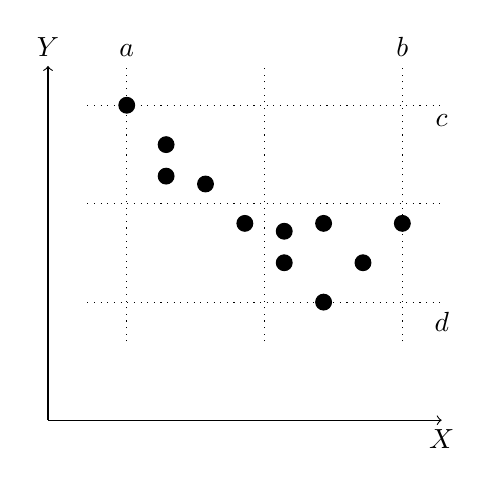
\begin{tikzpicture}      
		%\draw[help lines,xstep=.5,ystep=.5,dashed] (0,0) grid (6,6); %Hilfsdiagramm für Koordinaten
		%\foreach \x in {0,1 ,...,6} { \node [anchor=north] at (\x,0) {\x}; }
		%\foreach \y in {0,1,...,6} { \node [anchor=east] at (0,\y) {\y}; }
		
		\draw[->,] (0,0) -- 	(5,0) node  [at end,anchor= north]{$X$}; %x axis
		\draw[->,] (0,0) -- 	(0,4.5) node  [at end,anchor= south]{$Y$}; %z axis
		
		% sorted in rising x
		\draw[fill=black]       (1,4) circle (0.1) node (M)[below right]{}; % point M
		\draw[fill=black]       (1.5,3.5) circle (0.1) node (M)[below right]{}; % point M
		\draw[fill=black]       (1.5,3.1) circle (0.1) node (M)[below right]{}; % point M
		\draw[fill=black]       (2,3) circle (0.1) node (M)[below right]{}; % point M
		\draw[fill=black]       (2.5,2.5) circle (0.1) node (M)[below right]{}; % point M
		\draw[fill=black]       (3,2) circle (0.1) node (M)[below right]{}; % point M
		\draw[fill=black]       (3,2.4) circle (0.1) node (M)[below right]{}; % point M
		\draw[fill=black]       (3.5,1.5) circle (0.1) node (M)[below right]{}; % point M
		\draw[fill=black]       (3.5,2.5) circle (0.1) node (M)[below right]{}; % point M
		\draw[fill=black]       (4,2) circle (0.1) node (M)[below right]{}; % point M
		\draw[fill=black]       (4.5,2.5) circle (0.1) node (M)[below right]{}; % point M
	
		\draw[dotted] (1,1) -- 	(1,4.5) node  [at end,anchor= south]{$a$}; %left line
		\draw[dotted] (4.5,1) -- 	(4.5,4.5) node  [at end,anchor= south]{$b$}; %right line
		\draw[dotted] (0.5,1.5) -- 	(5,1.5) node  [at end,anchor= north]{$d$}; %bottom line
		\draw[dotted] (0.5,4) -- 	(5,4) node  [at end,anchor= north]{$c$}; %top line
		
		\draw[dotted] (0.5,2.75) -- 	(5,2.75) node  [at end,anchor= south]{}; %horizontal intersect
		\draw[dotted] (2.75,1) -- 	(2.75,4.5) node  [at end,anchor= north]{}; %vertical intersect
		
		
		\end{tikzpicture}
		\caption{Possible boxes to include data points of one cluster}
		\label{fig_lidarbox1}
	  \end{centering}
   	\end{minipage}\hfill
	\begin{minipage}[t]{0.48\textwidth}
	\begin{centering}
		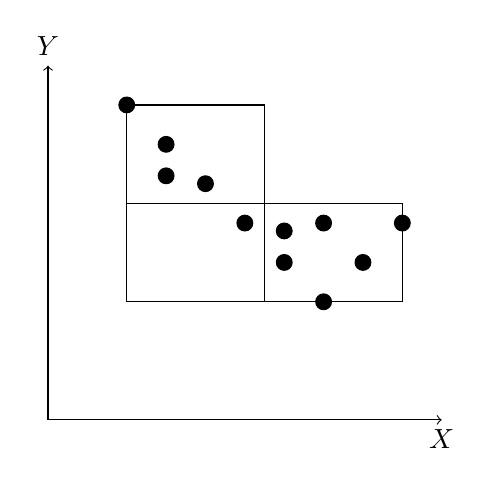
\begin{tikzpicture}      
		%\draw[help lines,xstep=.5,ystep=.5,dashed] (0,0) grid (6,6); %Hilfsdiagramm für Koordinaten
		%\foreach \x in {0,1 ,...,6} { \node [anchor=north] at (\x,0) {\x}; }
		%\foreach \y in {0,1,...,6} { \node [anchor=east] at (0,\y) {\y}; }
		
		\draw[->,] (0,0) -- 	(5,0) node  [at end,anchor= north]{$X$}; %x axis
		\draw[->,] (0,0) -- 	(0,4.5) node  [at end,anchor= south]{$Y$}; %z axis
		
		\draw[] (1,1.5) -- 	(1,4) node  [at end,anchor= south]{}; %left line
		\draw[] (4.5,1.5) -- 	(4.5,2.75) node  [at end,anchor= south]{}; %right line
		\draw[] (1,1.5) -- 	(4.5,1.5) node  [at end,anchor= north]{}; %bottom line
		\draw[] (1,4) -- 	(2.75,4) node  [at end,anchor= north]{}; %top line
		
		\draw[] (1,2.75) -- 	(4.5,2.75) node  [at end,anchor= south]{}; %horizontal intersect
		\draw[] (2.75,1.5) -- 	(2.75,4) node  [at end,anchor= north]{}; %vertical intersect
		
		% sorted in rising x
		\draw[fill=black]       (1,4) circle (0.1) node (M)[below right]{}; % point M
		\draw[fill=black]       (1.5,3.5) circle (0.1) node (M)[below right]{}; % point M
		\draw[fill=black]       (1.5,3.1) circle (0.1) node (M)[below right]{}; % point M
		\draw[fill=black]       (2,3) circle (0.1) node (M)[below right]{}; % point M
		\draw[fill=black]       (2.5,2.5) circle (0.1) node (M)[below right]{}; % point M
		\draw[fill=black]       (3,2) circle (0.1) node (M)[below right]{}; % point M
		\draw[fill=black]       (3,2.4) circle (0.1) node (M)[below right]{}; % point M
		\draw[fill=black]       (3.5,1.5) circle (0.1) node (M)[below right]{}; % point M
		\draw[fill=black]       (3.5,2.5) circle (0.1) node (M)[below right]{}; % point M
		\draw[fill=black]       (4,2) circle (0.1) node (M)[below right]{}; % point M
		\draw[fill=black]       (4.5,2.5) circle (0.1) node (M)[below right]{}; % point M
		\end{tikzpicture}
		\caption{Boxes resulting of discarded empty boxes of the cluster}
		\label{fig_lidarbox2}
	\end{centering}
\end{minipage}
\end{figure}
 
After receiving a \ac{RADAR} array with reflection values from Unity3d, its data is visualized in a \textit{matplotlib} plot in polar coordinate representation. Figure \ref{fig_RadarIntense} displays the resulting image. The byte typed array of reflection intensities is plotted for every cell from 0$\degree$ to 360$\degree$ with the according radius. To decrease the false alarm detection rate, a dynamic threshold is used in a next step to extract targets. The array that contains the detected signals is computed back to carthesian coordinates in order to obtain a general data format that was introduced by the \ac{LIDAR} data. It then is send to the \ac{ROS} network by taking the center of each detected signal.\\
 
In the scope of this work, only a two-dimensional collision mesh for the simulation of water is used and thus there are no wakes that can be falsely classified as a signal. Therefore the implementation of a \ac{OS-CFAR} algorithm is not required and the \ac{SOCA-CFAR} is used. However, in more sophisticated simulations or real world applications where situations can be expected in which many objects have to be detected that are in close proximity to each other, the \ac{OS-CFAR} is the algorithm of choice. Additionally, with the ability to model the strength of wakes with the Rayleigh \ac{PDF}, the \ac{OS-CFAR} provides further chances to reduce the false alarm rate.\\

Especially in artificially confined spaces with defined borders an algorithm that detect lines in the scenes images can provide useful information to specify the environment. In order to detect lines, the edges of the image have to be extracted. For that 
the python library OpenCV with a focus on real time applications for computer vision provides the so called Canny Edge Detection function. To extract edges, first a Gaussian filter is applied on the greyscale image to reduce noise. In a next step the edge gradients in vertical and horizontal directions are computed. The function allows for choosing the number of pixels that are included in the calculation for each gradient. If the gradient value is above a threshold one, the position is considered as an edge. If its below a threshold two, the value is discarded. For the values in between the two thresholds, the decision whether an edge is present or not is dependent on the existence of values above threshold two in the neighbourhood. The resulting edge image can be passed to the Hough-algorithm which then extracts the lines. Figure \ref{fig_Houghlines} visualizes the result of a line extraction applied to the image from the image sensor. Three blue lines indicate the detection of lines from an image, that has been passed to a edge detection beforehand. As the serialization of bytes is not implemented in the \textit{rosbridgelib} that connects Unity3d with ROS2, the image is saved in the underlying Linux filesystem. Only a message that indicates the availability of a new image and the place where it is saved is published in the ROS2 network. After the according \ac{ROS} node receives the message, the image is read from the specified storage place and can be processed.


\begin{figure}[!htb]
	\begin{minipage}[t]{0.48\textwidth}
		\centering
		\includegraphics[width=.9\linewidth]{Bilder/RadarIntensity.png}
		\caption{Radar data with reflection intensity}
		\label{fig_RadarIntense}
	\end{minipage}\hfill
	\begin{minipage}[t]{0.48\textwidth}
		\centering
		\includegraphics[width=.9\linewidth]{Bilder/houghlines.png}
		\caption{Edge image with visualized hough line detection in blue }
		\label{fig_Houghlines}
	\end{minipage}
\end{figure}

As a last step, the processed information of the \ac{LIDAR} and \ac{RADAR} are displayed together. Figure \ref{fig_RvizBird} displays the \ac{RADAR} data in red circles together with the \ac{LIDAR} data in yellow rectangles from a perspective above the scene. Figure \ref{fig_RvizThird} displays the same state of the scene from a third person perspective. The aforementioned bounding boxes of the \ac{LIDAR} data become visible in yellow with the size of a single box not exceeding a certain limit. The sensor center is indicated by  small coordinate system arrows in the center of the figure. Around the arrows the shape of the small vessel is displayed. The two dimensional \ac{RADAR} data is visualized with red cylinders. 
 \begin{figure}[!htb]
	\begin{minipage}[t]{0.48\textwidth}
		\centering
		\includegraphics[width=.9\linewidth]{Bilder/Objectmap.png}
		\caption{Lidar (yellow) and radar (red) objects from above}\label{fig_RvizBird}
	\end{minipage}\hfill
	\begin{minipage}[t]{0.48\textwidth}
		\centering
		\includegraphics[width=.9\linewidth]{Bilder/RvizThirdPerson.png}
		\caption{Lidar and radar objects in third person perspective}\label{fig_RvizThird}
	\end{minipage}
\end{figure}
%\begin{figure}
%	\centering
%	\includegraphics[width=10cm]{Bilder/Objectmap.png}
%	\caption{Lidar (yellow) and radar (red) objects from above}\label{fig_RvizBird}
%\end{figure}
%\begin{figure}
%\centering
%\includegraphics[width=10cm]{Bilder/RvizThirdPerson.png}
%\caption{Lidar and radar objects in third person perspective}\label{fig_RvizThird}
%\end{figure}


